\section{Embedding}
\subsection{Overview}
\begin{frame}[c]{We are here}
    \includegraphics[height=0.9\textheight]{Transformer_initial_embeddings}
\end{frame}

\begin{frame}[c]{Definitions}
    \large
    \begin{itemize}[<+(1)->]
        \item    \textbf{Vocabulary:} List of tokens available to the tokenizer, that can be recognized and generated \\
        \item    \textbf{Tokenizer:} Split the input apart using the available tokens in vocabulary \\
        \item    \textbf{Embedding:} Internal high-dimensional representation of given set of tokens (learned) \\
        % \item    \textbf{Mapping:} Individual tokens still need a mapping to an embedding (learned) \\
    \end{itemize}
    \pause
    The Vocabulary / Tokens are commonly learned via Byte Pair
    Encoding (BPE) \cite{shibata_byte_1999}. \\
\end{frame}

\subsection{Input Embedding}
\begin{frame}[c]{Input Embedding}
    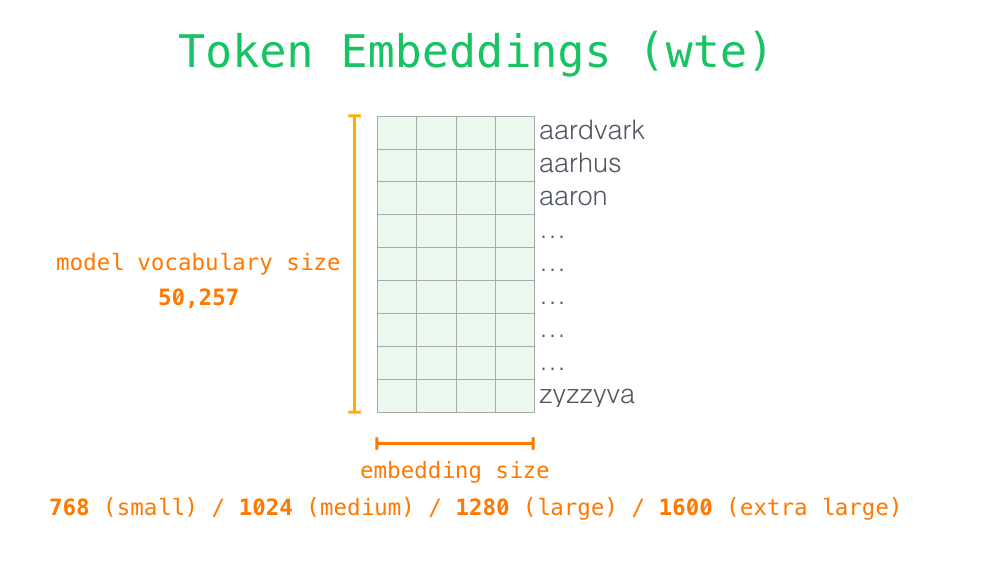
\includegraphics[width=\textwidth]{gpt2-token-embeddings-wte-2} \\
    \large
    Exemplary token to embedding encoding in GPT2.
    \normalsize
    Image Source: \cite{alammar_illustrated_2019}
\end{frame}

\begin{frame}[c]{In Code}
    \inputminted{python}{code/embedding.py}
    \todo{tokens not words}
\end{frame}

\subsection{Positional Encoding}

\begin{frame}[c]{Positional Encoding}
    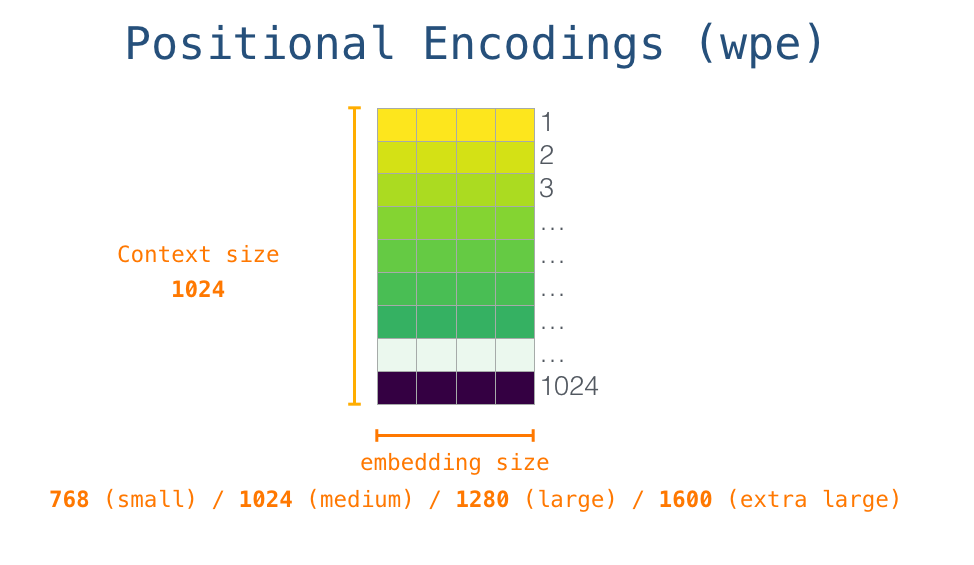
\includegraphics[width=\textwidth]{gpt2-positional-encoding} \\
    \large
    Exemplary positional encoding in GPT2. \\
    \normalsize
    Image Source: \cite{alammar_illustrated_2019}
\end{frame}

\begin{frame}[c]{Positional Encoding II}
    \large
    \textbf{Visualization} of a sinusoidal position encoding for the first 128 positions in 512 dimensions.
    \newline
    \newline
    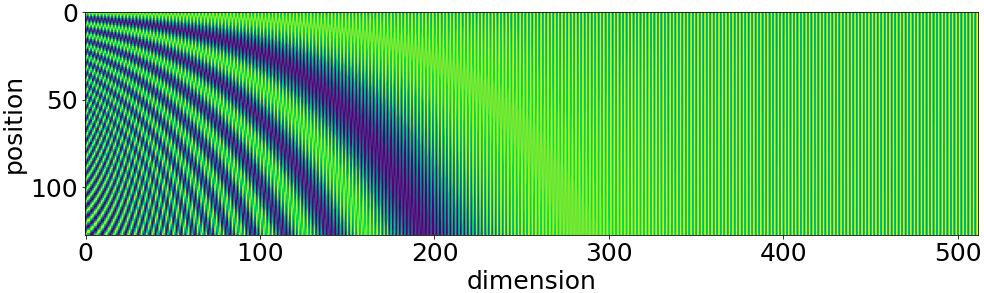
\includegraphics[width=\textwidth]{positional_encoding} \\
    \normalsize
    Image source: Public Domain
\end{frame}

\subsection{Full Input Embedding}
\begin{frame}[c]{Full Input Embedding}
    % trim=left bottom right top, clip
    \includegraphics[width=\textwidth,trim=0 0 0 700,clip]{Transformer_initial_embeddings}
    \large
    Simple Addition. Works well due to sparse high dimensional spaces.
\end{frame}


